\section{Đề số 38}

\begin{bt} 
	Tính các giá trị biểu thức sau:
	\\[5px]$A=\frac{\frac{1}{9}-\frac{1}{7}-\frac{1}{11}}{\frac{4}{9}-\frac{4}{7}-\frac{4}{11}}+\frac{0,6-\frac{3}{25}-\frac{3}{125}-\frac{3}{625}}{\frac{4}{5}-0,16-\frac{4}{125}-\frac{4}{625}}\\[5px]
	B=\frac{1-\frac{1}{\sqrt{49}}+\frac{1}{49}-\frac{1}{\left(7 \sqrt{7)^2}\right.}}{\frac{\sqrt{64}}{2}-\frac{4}{7}+\left(\frac{2}{7}\right)^2-\frac{4}{343}}$
	\loigiai{
		$\mathrm{A}=1\\[5px] 
		\mathrm{B}=\frac{1}{4}$
	} 
\end{bt}

\begin{bt}
	Tìm các số a a $_1, \mathrm{a}_2, \mathrm{a}_3, \ldots a_9$  biết
	$$
	\frac{a_1-1}{9}=\frac{a_2-2}{8}=\frac{a_3-3}{7}=\ldots=\frac{a_9-9}{1} \text { và } \mathrm{a}_1+\mathrm{a}_2+\mathrm{a}_3+\ldots+\mathrm{a}_9=90
	$$
	\loigiai{
		Áp dụng tính chất của dãy tỉ số bằng nhau ta tính được:\\[5px]
		$\mathrm{a}_1=\mathrm{a}_2=\ldots=\mathrm{a}_9=10$
	} 
\end{bt}

\begin{bt}
	\hfill 
	\begin{enumerate}[a.]
		\item Tìm x, y thoả mãn: $\quad\left|x^2+2 x\right|+\left|y^2-9\right|=0$
		\item Tìm $\mathrm{x}, \mathrm{y}$, z thoả mãn: $\sqrt{(x-\sqrt{2})^2}+\sqrt{(y+\sqrt{2})^2}+|x+y+z|=0$
	\end{enumerate}
	\loigiai{
		\begin{enumerate}
			\item Vì $\left|x^2+2 x\right| \geq 0$ và $\left|y^2-9\right| \geq 0 \Rightarrow \mathrm{x}^2+2 \mathrm{x}=0$ và $\mathrm{y}^2-9=0$ từ đó tìm được các cặp $(\mathrm{x} ; \mathrm{y})=$ $\{(0 ; 3) ;(0 ;-3) ;(-2 ; 3) ;(-2 ;-3)\}$
			\item Vì $\sqrt{(x-\sqrt{2})^2} \geq 0$ với $\forall \mathrm{x} ; \sqrt{(y+\sqrt{2})^2} \geq 0$ với $\forall \mathrm{y} ;|x+y+z| \geq 0$ với $\forall \mathrm{x}, \mathrm{y}, \mathrm{z}$\\[5px]
			Suy ra đẳng thức đã cho tương đương $\left\{\begin{array}{l}\sqrt{(x-\sqrt{2})^2}=0 \\[5px] \sqrt{(y+\sqrt{2})^2}=0 \\[5px] |x+y+x|=0\end{array}\\[5px] \Leftrightarrow\left\{\begin{array}{l}x=\sqrt{2} \\[5px] y=-\sqrt{2} \\[5px] z=0\end{array}\right.\right.$
		\end{enumerate}
	} 
\end{bt}

\begin{bt} 
	Cho $\frac{a}{c}=\frac{c}{b}$ chứng minh rằng: $\quad \frac{b^2-a^2}{a^2+c^2}=\frac{b-a}{a}$
	\loigiai{
		Từ $\frac{a}{c}=\frac{c}{b}$ suy ra $c^2=a . b$\\[5px] 
		khi đó $\frac{a^2+c^2}{b^2+c^2}=\frac{a^2+a \cdot b}{b^2+a \cdot b}=\frac{a(a+b)}{b(a+b)}=\frac{a}{b}$\\[5px] $\Rightarrow \frac{b^2+c^2}{a^2+c^2}=\frac{b}{a}$\\[5px]
		Từ $\frac{b^2+c^2}{a^2+c^2}=\frac{b}{a} \Rightarrow \frac{b^2+c^2}{a^2+c^2}-1=\frac{b}{a}-1$ hay $\frac{b^2+c^2-a^2-c^2}{a^2+c^2}=\frac{b-a}{a}$\\[5px] 
		Vậy $\frac{b^2-a^2}{a^2+c^2}=\frac{b-a}{a}$
	}
\end{bt}



\begin{bt}
	\hfill
	\begin{enumerate}[a.]
	\item Cho hàm số: $\quad y=f(x)=\left\{\begin{array}{l}x+1 \text { vói } x \geq-1 \\[5px] x-1 \text { với } x<-1\end{array}\right.$
	\begin{itemize}[-]
		\item Viết $\mathrm{f}(\mathrm{x})$ dưới dạng 1 biểu thức.
		\item Tìm $x$ khi $f(x)=2$.
		\item Tổng của 20 số đó là số âm.
	\end{itemize}
	\item Cho hai đa thức $P(x)=x^2+2 m x+m^2$ và $Q(x)=x^2+(2 m+1) x+m^2$ Tìm $\mathrm{m}$ biết $\mathrm{P}(1)=\mathrm{Q}(-1)$
	\end{enumerate}
	\loigiai{
		\begin{enumerate}
			\item Biểu thức xác định $\mathrm{f}(\mathrm{x})=|x+1|$\\[5px]
			Khi $\mathrm{f}(\mathrm{x})=2 \Rightarrow|x+1|=2$ từ đó tìm được $\mathrm{x}=1 ; \mathrm{x}=-3$.
			\item Thay giá trị tương ứng của $x$ vào 2 đa thức, ta tìm được biểu thức $P(1)$ và $Q(-1)$ theo $\mathrm{m}$ giải phương ẩn $\mathrm{m}$ mới tìm được\\[5px] $\Rightarrow \mathrm{m}=-\frac{1}{4}$
		\end{enumerate}
	}
\end{bt}

\begin{bt} 
	Tìm $\mathrm{x}, \mathrm{y}$ để $\mathrm{C}=-18-|2 x-6|-|3 y+9|$ đạt giá trị lớn nhất.
	\loigiai{
		Ta có $\mathrm{C}=-18-(|2 x-6|+|3 y+9|) \leq-18$\\[5px]
		$\text {Vì }|2 x-6| \geq 0 ;|3 y+9| \geq 0$\\[5px]
		Suy ra $C$ đạt giá trị lớn nhất bằng -18 khi $\left\{\begin{array}{l}2 x-6=0 \\[5px] 3 y+9=0\end{array}\right.$\\[5px]
		$\Rightarrow x=3 \text { và } y=-3$
	}
\end{bt}

\begin{bt} 
	Một ô tô chạy từ $\mathrm{A}$ đến $\mathrm{B}$ với vận tốc $65 \mathrm{~km} / \mathrm{h}$, cùng lúc đó một xe máy chạy từ $\mathrm{B}$ đến $\mathrm{A}$ với vận tốc $40 \mathrm{~km} / \mathrm{h}$. Biết khoảng cách $\mathrm{AB}$ là $540 \mathrm{~km}$ và $\mathrm{M}$ là trung điểm của $\mathrm{AB}$. Hỏi sau khi khởi hành bao lâu thì ô tô cách $\mathrm{M}$ một khoảng bằng $\frac{1}{2}$ khoảng cách từ xe máy đến M.
	\loigiai{
		$$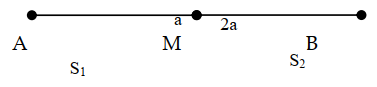
\includegraphics[width=0.45\textwidth]{38-7-lg.png}$$
		Quảng đường $\mathrm{AB}$ dài $540 \mathrm{~km}$, nửa quảng đường $\mathrm{AB}$ dài $270 \mathrm{~km}$.\\[5px]
		Gọi $\mathrm{t}$ là khoảng thời gian từ lúc khởi hành cho đến khi ô tô và xe máy lần lượt cách $\mathrm{M}$ bằng $\mathrm{a}$ và $2 \mathrm{a}(\mathrm{km}, \mathrm{a}>0)$.\\[5px]
		Khi đó ô tô và xe máy lần lượt đi được quảng đường là : 270 - a và 270 - 2a\\[5px]
		$\Rightarrow \mathrm{t}=\frac{270-a}{65}=\frac{270-2 a}{40} \\[5px]
		t=\frac{540-2 a}{130}=\frac{270-2 a}{40}=\frac{(540-2 a)-(270-2 a)}{130-40}=\frac{270}{90}=3$\\[5px]
		Vậy sau khi khởi hành 3 giờ thì ô tô cách $M$ một khoảng bằng $\frac{1}{2}$ khoảng cách từ xe máy tới $\mathrm{M}$.
	}
\end{bt}

\begin{bt}
	Cho $\triangle \mathrm{ABC}$ vuông cân ở $\mathrm{A}, \mathrm{M}$ là trung điểm của $\mathrm{BC}$, điểm $\mathrm{E}$ nằm giữa $\mathrm{M}$ và $C$. Kẻ $\mathrm{BH}, \mathrm{CK}$ vuông góc với $\mathrm{AE}(\mathrm{H}$ và $\mathrm{K}$ thuộc đường thẳng $\mathrm{AE})$. Chứng minh rằng:
	\begin{enumerate}[a.]
		\item $\mathrm{BH}=\mathrm{AK}$.
		\item $\triangle \mathrm{MBH}=\triangle \mathrm{MAK}$.
		\item $\Delta \mathrm{MHK}$ là tam giác vuông cân.
	\end{enumerate}
	\loigiai{
		$$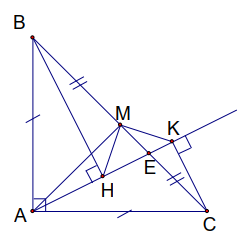
\includegraphics[width=0.4\textwidth]{38-8-lg.png}$$
		\begin{enumerate}
			\item Theo bài ra ta có: $\angle \mathrm{BAH}+\angle \mathrm{KAC}=\angle \mathrm{BAH}+\angle \mathrm{HBA}=>\mathrm{KAC}=\angle \mathrm{HBA}$\\[5px]
			$\text{mà } \mathrm{AB}=\mathrm{CA}(\mathrm{gt}) \\[5px]
			\Rightarrow \Delta \mathrm{HAB}=\Delta \mathrm{KCA}(\mathrm{ch}-\mathrm{gn}) \Rightarrow \mathrm{BH}=\mathrm{AK}$
			\item $\text{Có } ~ \angle \mathrm{MBH}+\angle \mathrm{HBA}=45^{\circ}=\angle \mathrm{MAK}+\angle \mathrm{KAC}$ mà $\angle \mathrm{KAC}=\angle \mathrm{HBA}$ (cm trên)\\[5px]
			$\Rightarrow \angle \mathrm{MBH}=\angle \mathrm{MAK}$\\[5px]
			Xét $\triangle \mathrm{MBH}$ và $\triangle \mathrm{MAK}$ có:\\[5px]
			$\mathrm{MB}=\mathrm{MA}(\mathrm{t} / \mathrm{c} \text { tam giác vuông }) \\[5px]
			\angle \mathrm{MBH}=\angle \mathrm{MAK}(\mathrm{c} / \mathrm{m} \text { trên }) \\[5px]
			\mathrm{BH}=\mathrm{AK}(\mathrm{c} / \mathrm{m} \text { trên }) \\[5px]
			\Rightarrow \Delta \mathrm{MBH}=\Delta \mathrm{MAK}(\text{đpcm})$
			\item Từ các kết quả trên $\Rightarrow \Delta \mathrm{MHA}=\Delta \mathrm{MKC}$ (c.c.c) và $\mathrm{MH}=\mathrm{MK}(1)$\\[5px] 
			$\Rightarrow \angle \mathrm{KMC}=\angle \mathrm{HMA}=>\angle \mathrm{KMC}+\angle \mathrm{CMH}=\angle \mathrm{HMA}+\angle \mathrm{CMH}=90^{\circ} \\[5px]
			\Rightarrow \angle \mathrm{HMK}=90^{\circ}(2)$\\[5px]
			Từ (1) và (2) $\Rightarrow \Delta \mathrm{MHK}$ vuông tại $\mathrm{M}($ (đpcm)
		\end{enumerate}
	}
\end{bt}
